\begin{frame}{Modelling}{Introduction}
	A model of the refrigeration system is derived, linearised and further developed for observer based control.
	\begin{itemize}
		\item \textbf{Main goal:} Capture dynamics important for the box air temperature (main control objective)
		\begin{itemize}
			\item Thermal masses: Trailer box, cargo, evaporator, condenser.
		\end{itemize}
		\item \textbf{Modular approach:} Inputs, outputs, internal equations/states
		\item \textbf{Slow vs. fast dynamics:} States or algebraic equations
		\begin{itemize}
			\item Including faster dynamics yield more accurate model yet it is unnecessary from control perspective.
		\end{itemize}		
	\end{itemize}
\end{frame}



%%%%%%%%%%%%%%%%%

\begin{frame}{Modelling}{Component Models}
	Each component is modelled separately. The components are:
	\begin{itemize}
		\item Expansion Valve
		\item Pipe joining junction
		\item Compressor
		\item Condenser
		\item Flash tank
		\item Evaporator
		\item Box
	\end{itemize}
\end{frame}



%%%%%%%%%%%%%%%%%

\begin{frame}{Modelling}{Expansion Valve}
	\textbf{Purpose:} Lower pressure of liquid refrigerant from flash tank to evaporator.
	\begin{itemize}
		\item Adiabatic process: Modelled algebraicly
		\item Inputs: Input pressure $p_{in}$, output pressure $p_{out}$, input enthalpy $h_{in}$
		\item Outputs: Flow through valve $\dot{m}$
	\end{itemize}
	
	\begin{equation} \label{eq:ExpansionValve_Alt}
		\begin{split}
			\dot{m} & = f_p(\Theta) K  \sqrt{\frac{1}{v_{in}} (p_{in} - p_{out})} \\
		\end{split}
	\end{equation}

	Table lookup:
	\begin{equation} \label{eq:ExpansionValve_vin}
		v_{in} = \mathcal{Z}(h_{in}, p_{in})
	\end{equation}
\end{frame}



%%%%%%%%%%%%%%%%%

\begin{frame}{Modelling}{Pipe joining junction}
	\textbf{Purpose:} Join refrigerant flows from between compressor stage 1 and two and the flash tank.
	\begin{itemize}
		\item Inputs: $\dot{m}_{in1}$, $\dot{m}_{in2}$, $\dot{m}_{out}$, $h_{in1}$ and $h_{in2}$
		\item Outputs: $h_{out}$
		\item States: $M$
	\end{itemize}
Mass balance:
	\begin{equation}
		 \frac{dM}{dt} = \dot{m}_{in1} + \dot{m}_{in2} - \dot{m}_{out}       \label{eq:PipeJoiningJunction_ChangeOfMass}
	\end{equation}
Enthalpy out:
\begin{equation} \label{eq:PipeJoiningJunction_Enthalpy}
	h_{out} = \frac{h_{in1} \cdot \dot{m}_{in1} + h_{in2} \cdot \dot{m}_{in2}}{ \dot{m}_{in1} + \dot{m}_{in2} }
\end{equation}
	
\end{frame}



%%%%%%%%%%%%%%%%%

\begin{frame}{Modelling}{Compressor}
	\textbf{Purpose:} Generate pressure sufficient for refrigerant flow and condenser heat flow
	\begin{itemize}
		\item Two compressor stages
		\item Only difference: Stage 2 has half the internal volume of stage 1
		\item Modelled as reciprocating (piston) compressor
		\item Modelled algebraicly - does not affect slow evaporator dynamics 
		\item Inputs: $p_{in}$, $T_{in}$ and $p_{out}$
		\item Outputs: $\dot{m}_{in}$, $\dot{m}_{out}$, $h_{out}$ and $T_{out}$
	\end{itemize}
Flow through compressor and enthalpy out
\begin{align}
	\dot{m} &= \left(\frac{V_1}{v_1} - \frac{V_C}{v_2}\right) \frac{\omega}{2} \label{eq:comp_mass_flow} \\
	h_{out} &= \Upsilon(T_{out}, p_{out}) \label{eq:comp_enthalpy}
\end{align}
\end{frame}

%%%%%%%%%%%%%%%%%

\begin{frame}{Modelling}{Condenser}
	\textbf{Purpose:} Exchange heat from hot vapour refrigerant to outside ambient air 
	\begin{itemize}
		\item Modelled as one Control Volume (CV)
		\item Inputs: $\dot{m}_{in}$, $h_{in}$ and $p_{out}$
		\item Outputs: $\dot{m}_{out}$, $h_{out}$ and $p_{in}$
		\item States: $M_r$ and $T_m$
	\end{itemize}
\begin{figure}[h!]
	\centering
	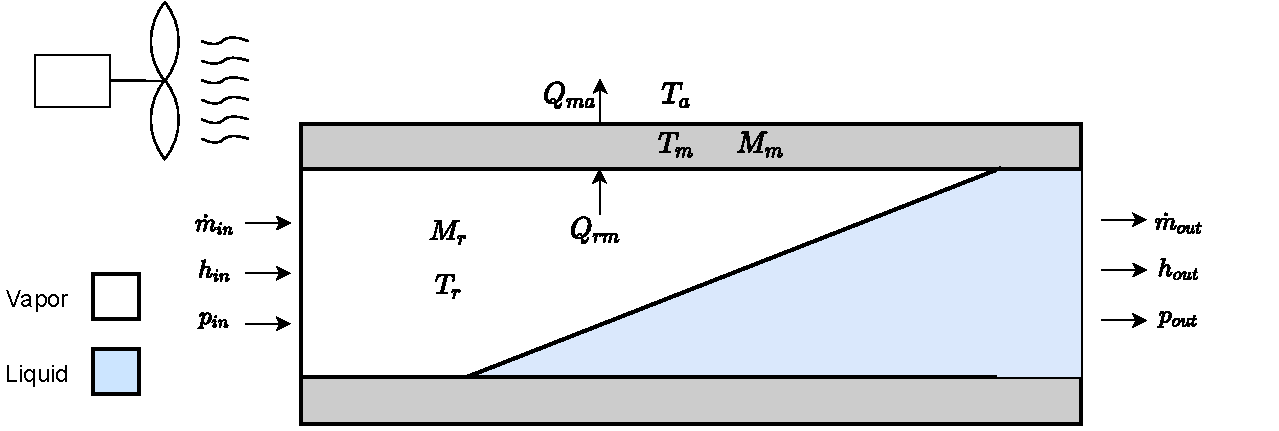
\includegraphics[width=1\textwidth]{../Graphics/Condenser.pdf}
	\caption{Diagram of condenser control volume}
	\label{fig:condenser_CV}
\end{figure}
\end{frame}

\begin{frame}{Condenser}{Equations}
	Energy balance:
	\begin{equation}
		h_{out} = h_{in} - \frac{Q_{rm}}{\dot{m}_{in}} \label{eq:Condenser_Enthalpy}
	\end{equation}
	Refrigerant mass balance:
	\begin{equation}
		\frac{dM_r}{dt} 	 = \dot{m}_{in}(t) - \dot{m}_{out}(t) \label{eq:Condenser_ChangeOfMass}
	\end{equation}
	Metal temperature:
	\begin{equation}
		\frac{dT_m}{dt} 	 = \frac{Q_{rm} - Q_{ma}}{M_m \cdot Cp_m} \label{eq:Condenser_ChangeOfTemperature}
	\end{equation}
\end{frame}




%%%%%%%%%%%%%%%%%

\begin{frame}{Modelling}{Flash tank}
	\textbf{Purpose:} Separate vapour and liquid refrigerant after condenser throttle valve (CDV)
	\begin{itemize}
		\item Modelled algebraicly
		\item Pressures out = in
		\item Inputs: $\dot{m}_{lv}$ and $\dot{m}_{l}$
		\item Outputs: $\dot{m}_{v}$, $h_l$ and $h_v$
	\end{itemize}
	\begin{figure}[h!]
		\centering
		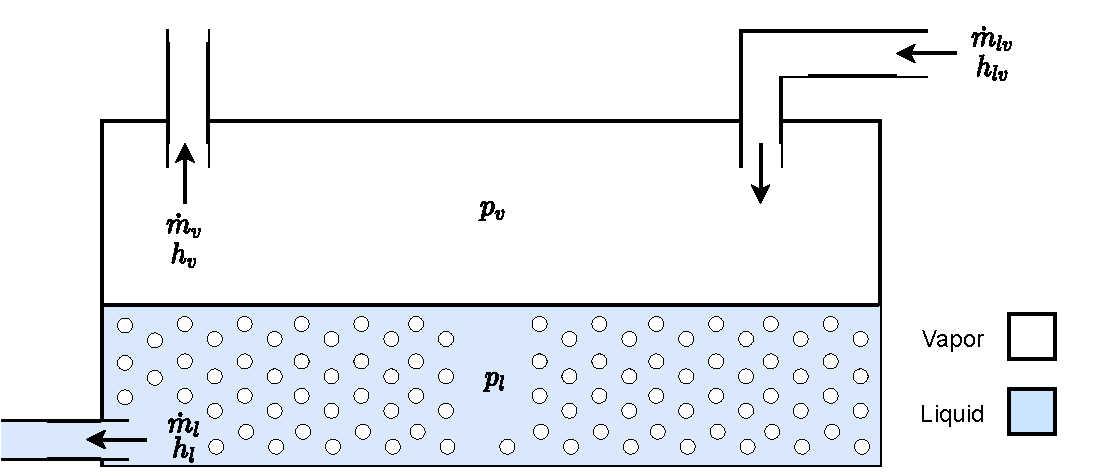
\includegraphics[width=0.8\textwidth]{../Graphics/Flash_tank.pdf}
		\caption{Diagram of Flash tank control volumes}
		\label{fig:flash_tank_CV}
	\end{figure}
\end{frame}

\begin{frame}{Flash tank}{Equations}
	Mass balance:
	\begin{equation}
		\dot{m}_{v} = \dot{m}_{lv} - \dot{m}_{l}  \label{eq:Flash_tank_massflow}
	\end{equation}
	Enthalpies:
	\begin{align}
		h_{l}  & = \mathcal{M}(p)\\
		h_{v}  & = \mathcal{N}(p)
	\end{align}
\end{frame}


%%%%%%%%%%%%%%%%%

\begin{frame}{Modelling}{Evaporator}
	\textbf{Purpose:} Exchange heat from box air to cold liquid refrigerant
	\begin{itemize}
		\item Superheat is important control objective
		\item Modelled with two CVs: liquid-vapour and vapour
		\item Pressure out is simplified to being pressure in
		\item Inputs: $p_{in}$, $\dot{m}_{in}$, $h_{in}$, $\dot{m}_{out}$, $T_{out}$ and $T_{ret}$
		\item Outputs: $p_{out}$, $h_{out}$ and $T_{sup}$
		\item States: $T_{mlv}$, $T_{mv}$, $M_{lv}$, $M_{v}$ and $T_{v}$
	\end{itemize}
	\begin{figure}[h!]
		\centering
		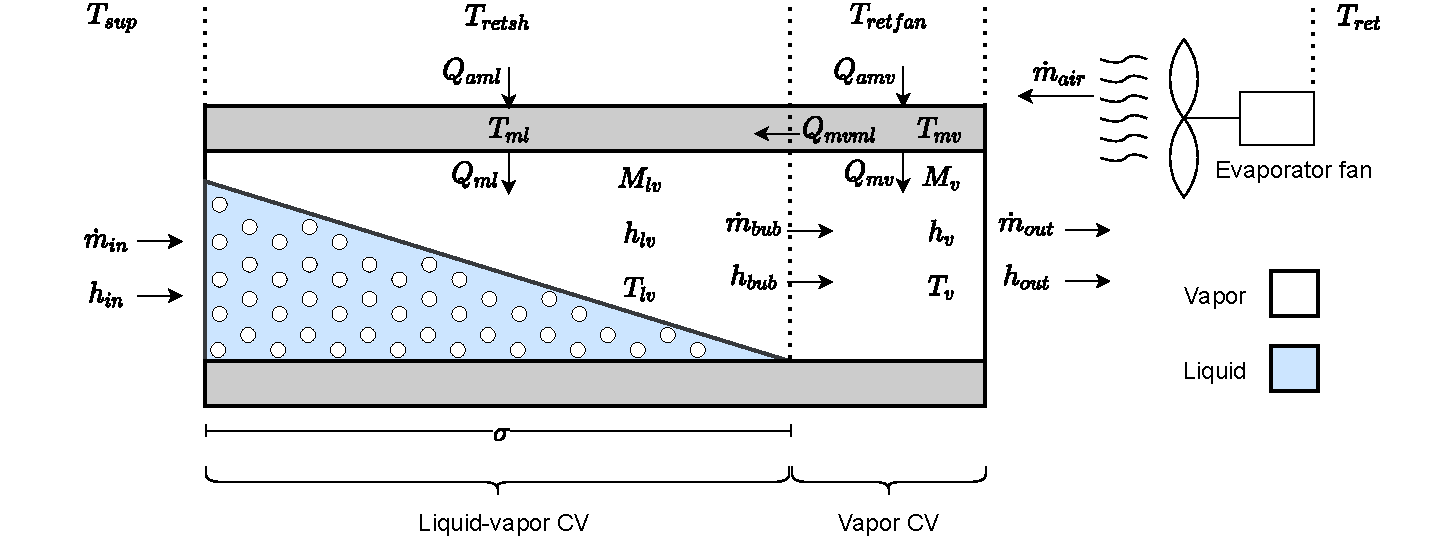
\includegraphics[width=1\textwidth]{../Graphics/Evaporator_CV_diagram.pdf}
		\caption{Diagram of evaporator liquid-vapour and liquid CVs split by $\sigma$}
		\label{fig:evap_CV}
	\end{figure}

\end{frame}

\begin{frame}{Evaporator}{Equations}
	Moving boundary and specific volume out
	\begin{equation}
		\sigma = \frac{M_{lv} \cdot v_1}{V_i} \label{eq:Evaporator_boundary}
	\end{equation}
	Liquid-vapour temperature:
	\begin{equation}
		\frac{dT_{mlv}}{dt}  = \frac{Q_{amlv}-Q_{mlv} + Q_{mvmlv}}{M_m \cdot \sigma \cdot Cp_m} \label{eq:evap_dT_ml}
	\end{equation}
	Vapour metal temperature:
	\begin{equation}
		\frac{dT_{mv}}{dt} = \frac{Q_{amv} - Q_{mv} - Q_{mvmlv}}{M_m \cdot (1 - \sigma) \cdot Cp_m} \label{eq:evap_dT_mv}
	\end{equation}
	Mass balances:
	\begin{equation} \label{eq:evap_dMlv}
		\frac{dM_{lv}}{dt} = \dot{m}_{in} - \dot{m}_{dew} \hspace{0.8cm}  \frac{dM_v}{dt} = \dot{m}_{dew} - \dot{m}_{out}
	\end{equation}
	Vapour refrigerant temperature:
	\begin{equation}\label{eq:tv_initial}
		\frac{dT_{v}}{dt} = \bar{T_v} - T_v
	\end{equation}

\end{frame}

%%%%%%%%%%%%%%%%%

\begin{frame}{Modelling}{Box}
	\textbf{Purpose:} Allow for convective heat transfer between cargo and circulating air
	\begin{itemize}
		\item Contains greatest thermal masses
		\item Inputs: $T_{sup}$
		\item Outputs: $T_{ret}$
		\item States: $T_{air}$, $T_{box}$ and $T_{cargo}$
	\end{itemize}
	\begin{figure}[h!]
		\centering
		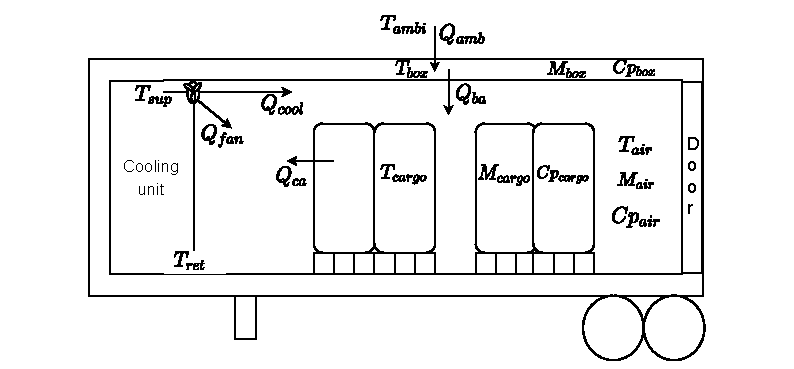
\includegraphics[width=0.8\textwidth]{../Graphics/Box.pdf}
		\caption{Simplified diagram of trailer box}
		\label{fig:box_diagram}
	\end{figure}


\end{frame}

\begin{frame}{Box}{Equations}
	Air, box and cargo temperatures:
	\begin{align}
		\frac{dT_{air}}{dt} &= \frac{Q_{ca} + Q_{ba} + Q_{fan} -Q_{cool}}{M_{air} \cdot Cp_{air}} \label{eq:box_dT_air} \\
		\frac{dT_{box}}{dt} &= \frac{Q_{amb} - Q_{ba}}{M_{box} \cdot Cp_{box}} \label{eq:box_dT_box} \\
		\frac{dT_{cargo}}{dt} &= \frac{-Q_{ca}}{M_{cargo} \cdot Cp_{cargo}} \label{eq:box_dT_cargo}
	\end{align}
	Heat flows:
	\begin{align}
		Q_{cool}   & = Cp_{air} \cdot \dot{m}_{air} \cdot (T_{ret} - T_{sup})	\label{eq:box_Qcool} \\
		Q_{amb}    & = (T_{ambi} - T_{box}) \cdot U A_{amb}						\label{eq:box_Qab}   \\
		Q_{ba}     & = (T_{box} - T_{air}) \cdot U A_{ba}						\label{eq:box_Qba}   \\
		Q_{ca}     & = (T_{cargo} - T_{air}) \cdot U A_{ca}                  	\label{eq:box_Qca}
	\end{align}
\end{frame}

%%%%%%%%%%%%%%%%%

\begin{frame}{Modelling}{}
	\textbf{Purpose:} 
	\begin{itemize}
		\item Inputs: 
		\item Outputs: 
		\item States: 
	\end{itemize}


\end{frame}



%%%%%%%%%%%%%%%%%

\begin{frame}{Modelling}{}
	
\end{frame}



%%%%%%%%%%%%%%%%%



